% !TEX root = main.tex
% !TEX encoding = UTF-8

\chapter{Model Design for SystemBuilder} \label{sec:model_design}

After generating and training a network in NNC, we convert the model for SystemBuilder to implement on FPGA. This chapter will discuss this model design for SystemBuilder using network structure and trained parameters from NNC.

\section{Overall Design} \label{sec:overall_design}

\begin{figure}[tbp]
  \centering
  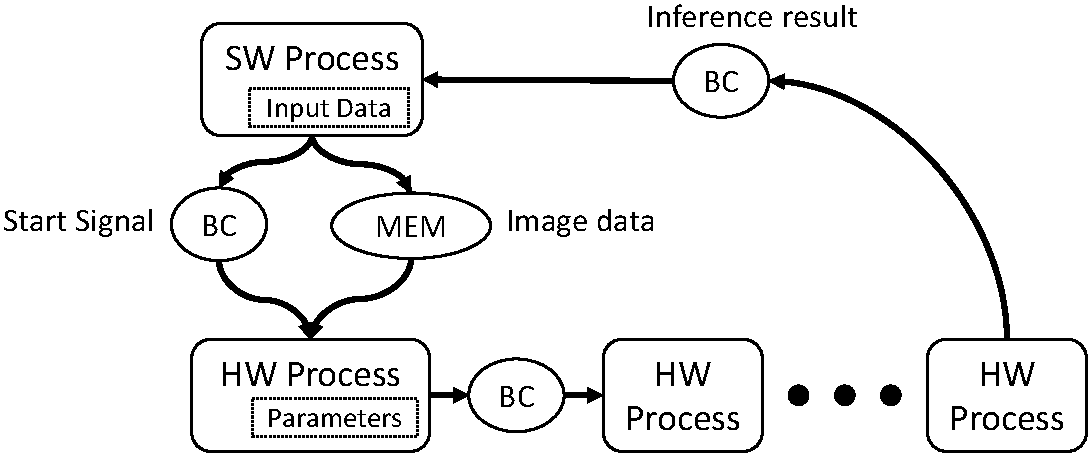
\includegraphics[width=0.82\linewidth]{designed_architecture.pdf}
  \caption{Overall design of the implemented model}%
  \label{fig:designed_architecture}
\end{figure}

To use SystemBuilder, we write the System DeFinition (SDF) file that describes the overall model design. \Figref{fig:designed_architecture} is the example showing the SDF file we designed.
Communication primitives are represented as an ellipse, and functional units are represented as a rounded rectangle. The arrow leaving the unit represents the write function toward the communication primitive, and the incoming arrow represents the read function of the communication primitive. We use memory primitive to send input data to a hardware process and blocking channel primitive to send start signal and receive the inference result. If multiple hardware processes are declared as \Figref{fig:designed_architecture}, we use blocking channel primitive to communicate between hardware processes. \Figref{fig:eg_sdf} is a part of the SDF file we designed.

The input data is prepared as text and read as a global array variable in the software process, and the parameters are also prepared as text and used as global variables in each layer code.

% Software process sends start signal using BC, send image data with memory primitive, and receive inference result with BC. We designed a software process to measure the time it takes from the sending start signal to the arrival of the result. For the hardware processes, we designed it to receive the input image data and return the inference value to the software. In the case of using multiple hardware processes, we used BC as the communication primitives between hardware processes. The reason and method for using several hardware processes will be discussed in section \ref{sec:design_case_study}.



As shown in \Figref{fig:designed_architecture}, the hardware returns inferred result to SW process from the received data. For hardware process design, we take two approaches.

\paragraph{Design 1}

\begin{figure}[tbp]
  \centering
  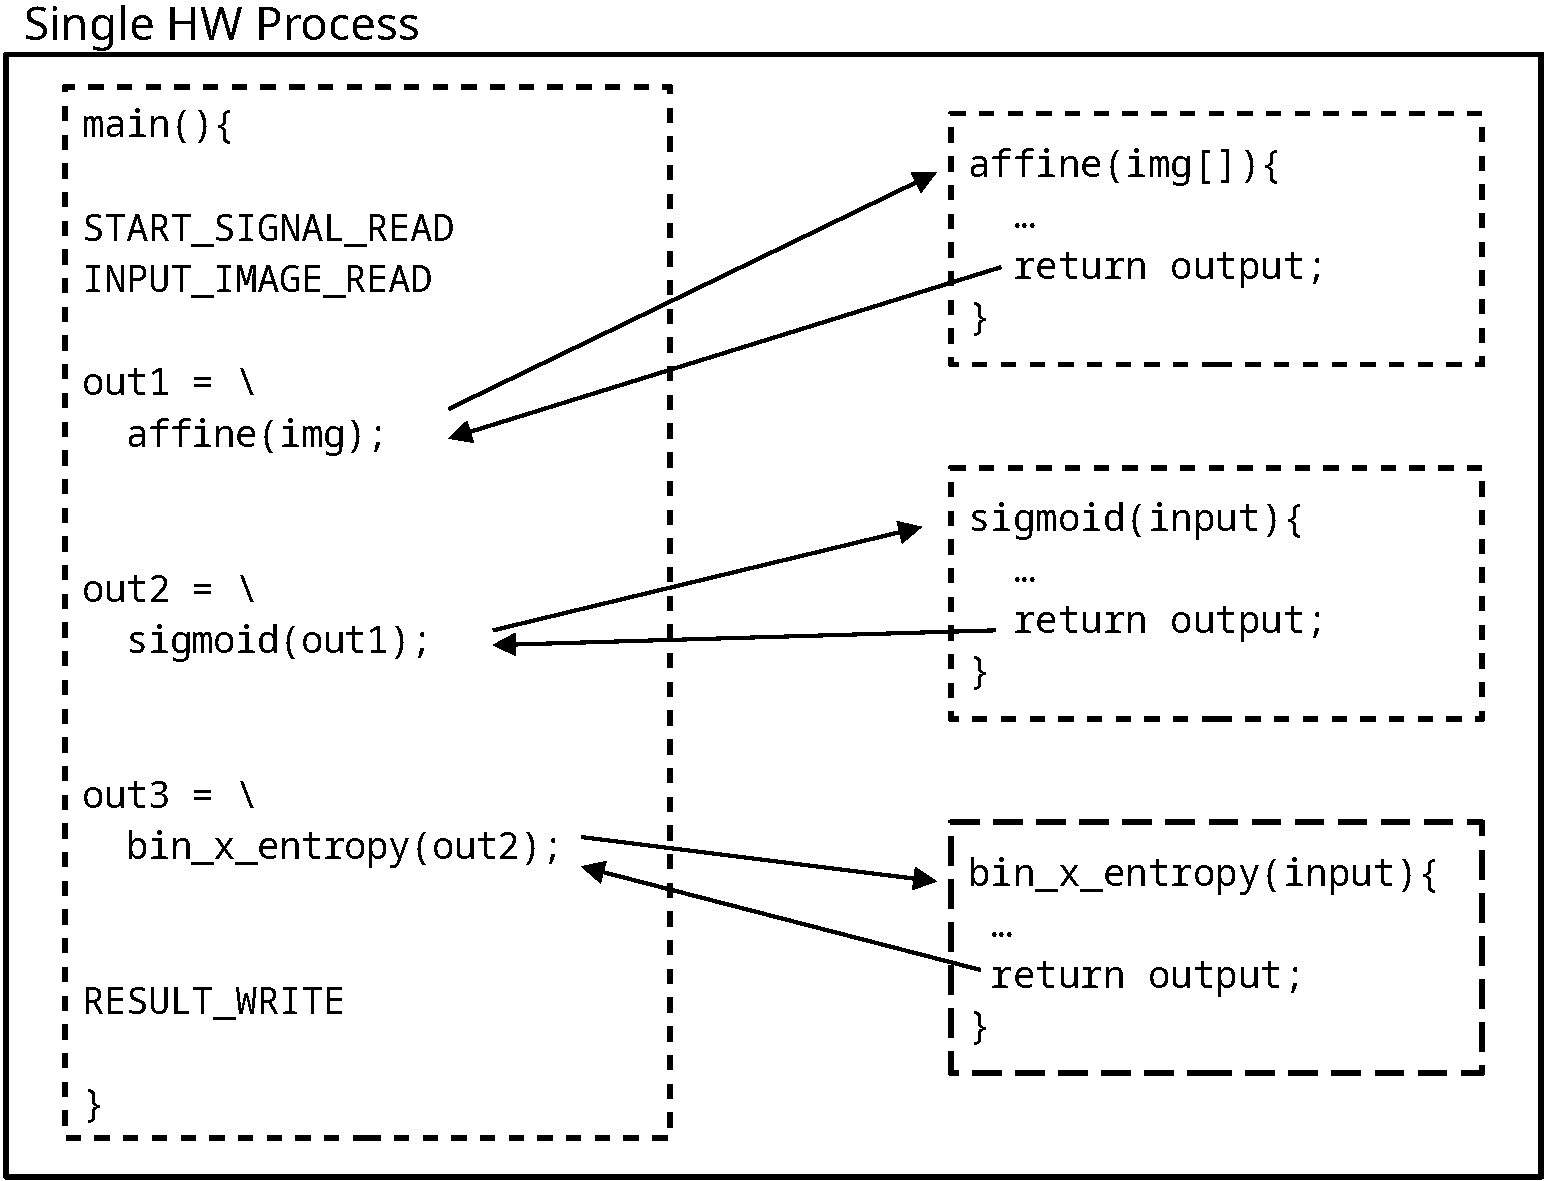
\includegraphics[scale=0.44]{hw_process_desgin_case1.pdf}
  \caption{Single hardware process}%
  \label{fig:hw_design_1}
\end{figure}

The first approach uses a single hardware process, as shown in \Figref{fig:hw_design_1}. In this single process, several functions that play each layer's role are declared. It operates by calling each function inside the hardware process's primary function.

\paragraph{Design 2}

\begin{figure}[tbp]
  \centering
  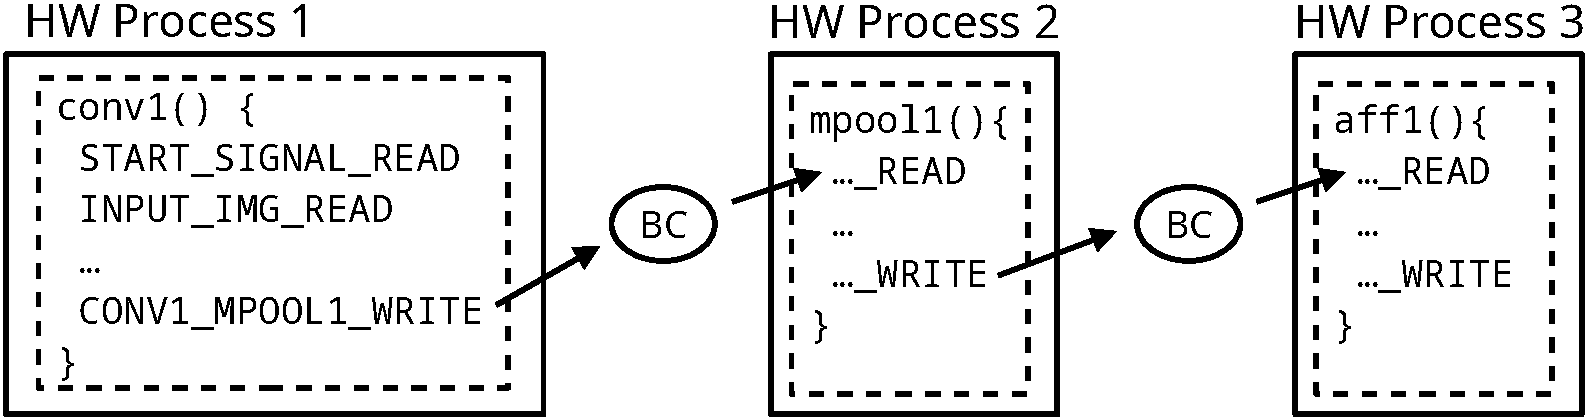
\includegraphics[scale=0.44]{hw_process_desgin_case2.pdf}
  \caption{Multiple hardware processes}%
  \label{fig:hw_design_2}
\end{figure}

The second approach uses several hardware processes, as shown in \Figref{fig:hw_design_2}. Each process has a single function that plays the role of each layer. However, not all layer is created as a process. We create a process that corresponds to the convolution, affine, and max-pooling layers. These layers are layers that have different sizes of input data and output data. The other layers, such as an activation layer, will be built-in in the previous layer's process. For example, if one matrix element is calculated in the convolution operation, this element value passes through the activation function and is sent to the next layer.

Each process transfers one element of the resulting matrix to the next process as it is computed. The next process receives input results and then operate. Data transfer between hardware processes uses blocking channel primitive.

\section{Design of each layer}
In the previous section, we discussed the overall model design. We also discussed how the hardware processes are configured. This section will discuss the actual implemented design of three-layer, convolution, affine, and max-pooling. These layers are separately designed to be hardware process in \textbf{Design 2} of section \ref{sec:overall_design}.

We will discuss the design using the pseudocode. However, addition and multiplication in the pseudocode used are far from real. Since we are handling quantized numbers in the implementation, we take different addition and multiplication method, which will be discussed in section \ref{sec:implementation_operations}.

\subsection{Convolution}
The following code is pseudocode for the convolution layer.

\begin{quote}
\begin{lstlisting}[language=C, frame=l]
Receive results from the previous process

for (o_ch = 0; o_ch < output_channel; ++o_ch){
    for (o_h = 0; o_h < output_height; ++o_h){
        for (o_w = 0; o_w < output_width; ++o_w){

            result = 0;
            for (k_d = 0; k_d < kernel_dimension; ++k_d){
                for (k_h = 0; k_h < kernel_height; ++k_h){
                    for (k_w = 0; k_w < kernel_width; ++k_w){
                        result += input_element * kernel_element;
                    }
                }
            }
            // add bias
            result += bias_element;

            Modify result if needed (e.g. activation function)
            Print result
        }
    }
}
\end{lstlisting}


\end{quote}

The convolution layer is a layer that adds a bias to the sum of matrices multiplications. The triple for statement calculates each element of the output matrix sequentially  (line 3--5). In the inner triple loop, we access each element of the input and the kernel (line 8--10). Then, we calculate the sum of the accessed elements' multiplications (line 11) and add a bias (line 16). Next, as we discussed in section \ref{sec:overall_design}, we built some layers in one of the two hardware designs, such as an activation layer in its previous layer. In this case, it is processed (line 18). Then finally, the code print the output element (line 19).

% the if processing such as an activation function is needed, it is processed (line 18).

\subsection{Affine}
The following code is pseudocode for the affine layer.

\begin{quote}
\begin{lstlisting}[language=C, frame=l]
Receive results from the previous process

for (ch = 0; ch < output_channel; ++ch){
    result = 0;
    for (i = 0; i < input_size; ++i){
        result += input_element * parameter_element;
    }
    // add bias
    result += bias_element;

    Modify the result if needed (e.g. activation function)
    Print the result
}
\end{lstlisting}
\end{quote}

% The affine layer is a layer that adds a bias to the matrices multiplications, .

An affine layer is written in a structure similar to the convolution layer. The outer for statement calculates each output matrix element sequentially (line 3). Inner for statement calculates the sum of the multiplications (line 5--7). Like the convolution layer, after adding the bias (line 9), we modify the result if needed and print the result (line 11--12).

\subsection{Max-pooling}
The following code is pseudocode for the max-pooling layer.
\begin{quote}
\begin{lstlisting}[language=C, frame=l]
Receive results from the previous process

for (o_ch = 0; o_ch < output_channel; ++o_ch){
    for (o_h = 0; o_h < output_height; ++o_h){
        for (o_w = 0; o_w < output_width; ++o_w){

            local_max = -128;
            for (k_h = 0; h < kernel_height; ++k_h){
                for (k_w = 0; w < kernel_width; ++k_w){
                    temp = input_element;
                    if (temp > local_max) {
                        local_max = temp;
                    }
                }
            }

            Modify the local_max if needed (e.g. activation function)
            Print the local_max
        }
    }
}
\end{lstlisting}
\end{quote}

Like other designs described above, the code calculates each element of the output matrix sequentially using for statement (line 3--5). Next, it founds the largest element within the range specified by the kernel using double for statement (line 7--15). Like other designs, we modify the result and print the result (line 17--18).

% After modifying the result if needed (line 17), it print the result (line 18).



\section{Implementation of operations with quantized data}\label{sec:implementation_operations}

As discussed in section \ref{sec:nnc}, the FixedPointQuantize layer's output is a float in NNC. Therefore the other layer can be a generic usable design without considering the input is quantized or not.
% However, as we will cover in section \ref{sec:quantization}, we wanted to eliminate the use of floating-point arithmetic from our models. Therefore, we should design the layers to handle only an integer type.
However, we want to eliminate the use of floating-point arithmetic from our models. Therefore, we should design the layers to handle only an integer type.

Since we set the quantization step size ($\delta$) as the power of two, data can be expressed as follows:
% \begin{equation} % \label{eq:quant}
\[
\textrm{quantized data in original scale} = \textrm{quantized data} \times \delta, \quad \delta = 2^{-n} \; \left( n = 1, 2, \ldots\right)
\]

While `quantized data' is an integer value and $\delta$ is the quantization step.

Our model only handles this `quantized data'. Therefore, rather than the concept of passing the float data through the FixedPointQuantize layer like NNC, we designed other layers to include the concept of FixedPointQuantize layer.

Each layer receives the quantized integer as input and outputs as an integer. Quantization steps of input, output, and parameters can be different. Consequently, we take this into account when designing. This subsection will cover the implemented methods of operations with quantized data.

% , but in our model, the output of each layer is an integer with  so we have to take a slightly different approach.

\subsubsection{Addition}
Let $a$ and $b$ be defined as quantized numbers, and let $A$ and $B$ be values expressed in the original scale of $a$ and $b$. The following equations express these relations.

\begin{align*}
  A &= a \times \delta_a \\
  B &= b \times \delta_b
\end{align*}

 Since we use delta as the power of two in our implementation, let us also define $\delta_a$ and $\delta_b$ as the following equations.

\begin{align*}
  \delta_a & = 2 ^{-\alpha} \\
  \delta_b & = 2^{-\beta} \\
  \alpha,\; \beta & \in \textbf{Z}
\end{align*}

$A + B$ will be expressed as the following equation.

\begin{align*}
  A + B &= (a \times 2^{\beta - \alpha} + b) \times 2^{-\beta}
\end{align*}

Assume, without loss of generality, that $\delta_a$ is greater than or equal to $\delta_b$. Then $a \times 2^{\beta - \alpha} + b$ will be an integer. This value will be the result of the addition between quantized numbers. This value has the following meanings: The result is the addition between $a$ with adjusted quantization step and $b$. The result's quantization step will be a lower value among the operand's quantization step, which is $2^{-\beta}$ in the above equation. The following codes can express this process in the implementation.

\begin{quote}
  \lstinputlisting[language=C, numbers=left, frame=l]{"src/impl_addition.c"}
  % \caption{Implementation of addition}
  % \label{fig:addition}
\end{quote}

To decrease $a$'s quantization step by divided by $2^{\beta - \alpha}$, we increased $a$ multiplied by $2^{\beta - \alpha}$. To maximize the performance, we use a bitwise shift operation. The behavior of bitwise left shift operation with a negative number is undefined in C standard \cite{iso:c17}. Therefore, we use the if statement as line 2 to determine the negative number to solve this problem.

Variable `\texttt{a\_alter}' and `\texttt{result}' should be declared in wide-enough data type to avoid integer overflow in operation.

\subsubsection{Multiplication}

Let $a$ and $b$ use the same definition as in \textbf{Addition}. Multiplication of $a$ and $b$ can be expressed as the following equation.

\begin{align*}
  AB &= a b\times (\delta_a \times \delta_b)
\end{align*}

This equation means the result of a multiplication is $a\times b$, and the quantization step size will be the multiplication of the operand's quantization step. The following codes can express the multiplication in the implementation.

\begin{quote}
  \begin{lstlisting}[language=C, numbers=left, frame=l]
result = ((int32_t) a) * b;
  \end{lstlisting}
\end{quote}
  % \caption{Implementation of multiplication}%
  % \label{fig:multiplication}

% Multiplication can be expressed as \Figref{fig:multiplication} in the implementation.

We typecast the variable to wider data types to avoid overflow. Moreover, the variable `\texttt{result}' should be declared in a wider data type.

\subsubsection{Typecasting to narrower data types}

We store the operation result in a wider data type to implement addition and multiplication. We use a 32-bit integer to store the operation value during the process. After performing the operation required by each layer, typecasting to narrower data types is required. Each layer's output should be quantized to an 8-bit integer, not 32-bit. Moreover, we should also adjust the number's quantization step to match the output's one.



% \begin{figure}
%   \centering
%   \lstinputlisting[
%     language=C
%   ]{"src/impl_typecasting.c"}
%   \caption{Implementation of typecasting}
%   \label{fig:typecasting}
% \end{figure}

To perform this process, we use the following steps. First, we change the quantization step to match layer output. Second, we check the overflow and underflow.

% Which can be expressed as the following codes \Figref{fig:typecasting} in the implementation. In this code, we quantize variable \texttt{result} to \texttt{output}.

\paragraph{Step 1}
Changing the quantization step can be expressed as the following codes in the implementation. % In this code, we quantize variable \texttt{result} to \texttt{output}.
\begin{quote}
  \lstinputlisting[
  language=C,
  numbers=left,
  frame=l,
  linerange={1-7},
  firstnumber=1,
  ]{"src/impl_typecasting.c"}
\end{quote}

% Lines 1 to 7 are the code to change the quantization step.

In the code, it increases the quantization step by multiplied by $2^{\texttt{rescale\_amount}}$. We use the right shift operation to accomplish it. Since the right shift operation will truncate the \texttt{result}, we added a number to round it (line 2 and 5). For example, let us apply the code above to the following variable:
\begin{quote}
  \texttt{result} $=$ \texttt{0b 0100 0100}\\
  \texttt{rescale\_amount} $=$ \texttt{4}
\end{quote}
The variable `\texttt{result}' then will be ``\texttt{0b 0000 0101}''.

% Suppose we need to decrease the quantization step. In that case,
In the case of decreasing the quantization step, we can use the left shift operation method described in \textbf{Addition}. However, in the case study, the quantization step of the output always has been large or equal to the quantization step of an internal variable like `\texttt{result}'.

\subparagraph{An equivalent code in NNC}
An equivalent task happens in NNC. \Figref{fig:fixedpointquantize} is the part of the source code of the FixedPointQuantize layer. The equivalent part is line 59 -- 62 of this figure.

\begin{itemize}
  \item The concept that determines the sign of `\texttt{result}' in our model (if statement in line 1) is equivalent to lines 59, 60, and 62 of \Figref{fig:fixedpointquantize}. We design to divide the case with an if statement, but developers of NNC designs to handle with absolute values first and then handle sign next.

  \item The concept avoids truncating while left shifting is implemented in lines 2 and 5 on our models. This is equivalent to line 61 of \Figref{fig:fixedpointquantize}. The developers of NNC designs to add $0.5$ before the multiplication of quantization step (\texttt{delta\_}).
\end{itemize}


\paragraph{Step 2} Checking the overflow and underflow can be expressed as the following codes in the implementation.

\begin{quote}
  \lstinputlisting[
  language=C,
  numbers=left,
  frame=l,
  linerange={9-15},
  firstnumber=1,
  ]{"src/impl_typecasting.c"}
\end{quote}

Where \texttt{MIN} is a minimal value, and \texttt{MAX} is a maximum value of \texttt{output}'s data type. For example, if \texttt{output} is declared in an unsigned 8-bit integer, it will be \texttt{0} and \texttt{255}. Furthermore, if \texttt{output} is declared in a signed 8-bit integer, it will be \texttt{-128} and \texttt{127}.

\subparagraph{An equivalent code in NNC}
An equivalent part in NNC is line 54 -- 57 in \Figref{fig:fixedpointquantize}. However, in NNC, checking the overflow and underflow can be performed before step 1 process because the input and output are on the same scale.

% Variable \texttt{result} is 32-bit integer in our models, which can have lower quantization step compare to 8-bit integer. Therefore we did not used that method.
